\chapter{Anomaly detection: Taxi calls}

\begin{description}
    \item[Anomaly] \marginnote{Anomaly}
        Event that deviates from the usual pattern.

    \item[Time series] \marginnote{Time series}
        Data with an ordering (e.g., chronological).
\end{description}



\section{Data}

The dataset is a time series and it is a \texttt{DataFrame} with the following fields:
\begin{descriptionlist}
    \item[\texttt{timestamp}] with a 30 minutes granularity.
    \item[\texttt{value}] number of calls.
\end{descriptionlist}

The label is a \texttt{Series} containing the timestamps of the anomalies.

An additional \texttt{DataFrame} contains information about the time window in which the anomalies happen:
\begin{descriptionlist}
    \item[\texttt{begin}] acceptable moment from which an anomaly can be detected.
    \item[\texttt{end}] acceptable moment from which there are no anomalies anymore.
\end{descriptionlist}

\begin{figure}[H]
    \centering
    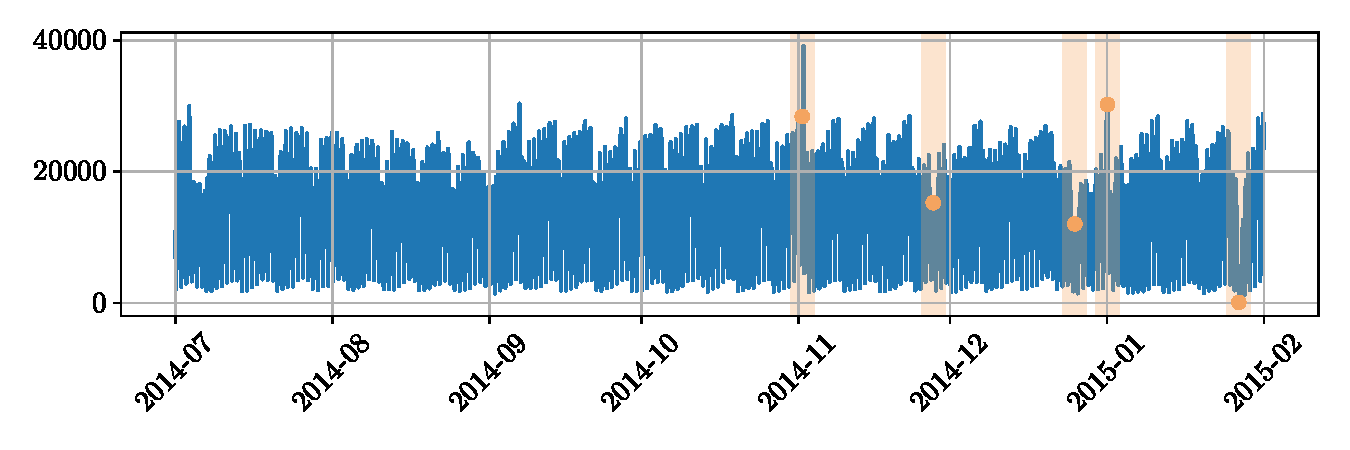
\includegraphics[width=0.7\linewidth]{./img/_ad_taxi_data.pdf}
    \caption{Plot of the time series, anomalies, and windows}
\end{figure}



\section{Approaches}


\subsection{Gaussian assumption}

Assuming that the data follows a Gaussian distribution, mean and variance can be used to determine anomalies through a threshold. $z$-score can also be used.


\subsection{Characterize data distribution}

Classify a data point as an anomaly if it is too unlikely.

\begin{description}
    \item[Problem formalization] 
        Given a random variable $X$ with values $x$ to represent the number of taxi calls, we want to find its probability density function (PDF) $f(x)$.

        An anomaly is determined whether:
        \[ f(x) \leq \varepsilon \]
        where $\varepsilon$ is a threshold.

        \begin{remark}
            A PDF can be reasonably used even though the dataset is discrete if its data points are sufficiently fine-grained.
        \end{remark}

        \begin{remark}
            It is handy to use negated log probabilities as:
            \begin{itemize}
                \item The logarithm adds numerical stability.
                \item The negation makes the probability an alarm signal, which is a more common measure.
            \end{itemize}
            Therefore, the detection condition becomes:
            \[ - \log f(x) \geq \varepsilon \]
        \end{remark}

    \item[Solution formalization]
        The problem can be tackled using a density estimation technique.
\end{description}


\subsubsection{Univariate kernel density estimation}

\begin{description}
    \item[Kernel density estimation (KDE)] \marginnote{Kernel density estimation (KDE)}
        Based on the assumption that whether there is a data point, there are more around it. Therefore, each data point is the center of a density kernel.

        \begin{description}
            \item[Density kernel] 
                A kernel $K(x, h)$ is defined by:
                \begin{itemize}
                    \item The input variable $x$.
                    \item The bandwidth $h$.
                \end{itemize}
        
                \begin{description}
                    \item[Gaussian kernel]
                        Kernel defined as:
                        \[ K(x, h) \propto e^{-\frac{x^2}{2h^2}} \]
                        where:
                        \begin{itemize}
                            \item The mean is $0$.
                            \item $h$ is the standard deviation.
                        \end{itemize}
                        As the mean is $0$, an affine transformation can be used to center the kernel on a data point $\mu$ as $K(x - \mu, h)$.
                \end{description}
        \end{description}

        Given $m$ training data points $\bar{x}_i$, the density of any point $x$ can be computed as the kernel average:
        \[ f(x, \bar{x}, h) = \frac{1}{m} \sum_{i=0}^{m} K(x - \bar{x}_i, h) \]

        Therefore, the train data themselves are used as the parameters of the model while the bandwidth $h$ has to be estimated. 

        \begin{remark}
            According to some statistical arguments, a rule-of-thumb to estimate $h$ in the univariate case is the following:
            \[ h = 0.9 \cdot \min\left\{ \hat{\sigma}, \frac{\texttt{IQR}}{1.34} \right\} \cdot m^{-\frac{1}{5}} \]
            where:
            \begin{itemize}
                \item $\texttt{IQR}$ is the inter-quartile range.
                \item $\hat{\sigma}$ is the standard deviation computed over the whole dataset.
            \end{itemize}
        \end{remark}

    \item[Data split] 
        Time series are usually split chronologically:
        \begin{descriptionlist}
            \item[Train] Should ideally contain only data representing the normal pattern. A small amount of anomalies might be tolerated as they have low probabilities.
            \item[Validation] Used to find the threshold $\varepsilon$.
            \item[Test] Used to evaluate the model.
        \end{descriptionlist}

        \begin{figure}[H]
            \centering
            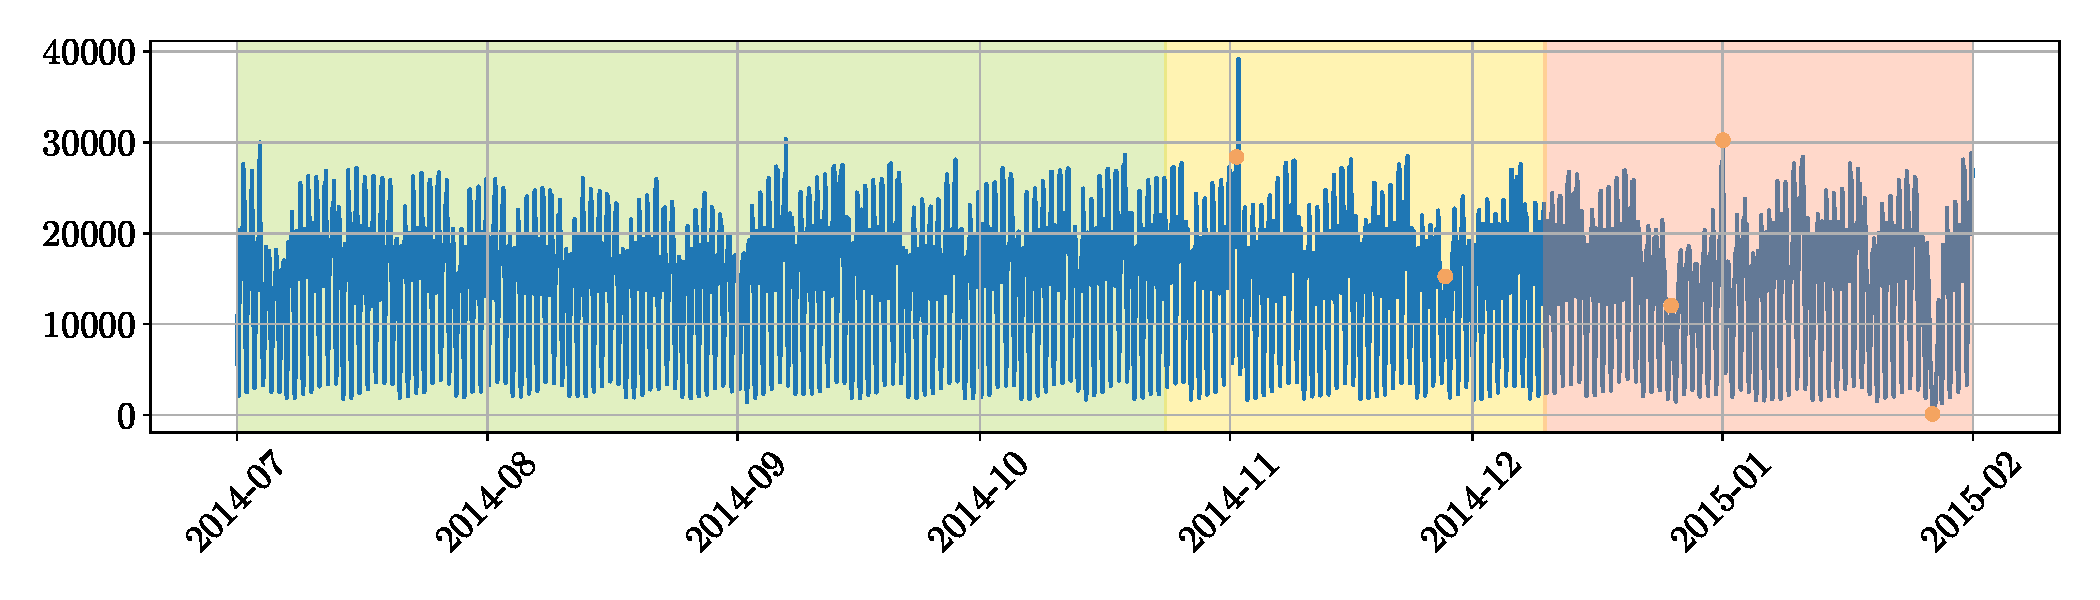
\includegraphics[width=0.8\linewidth]{./img/_ad_taxi_splits.pdf}
            \caption{Train, validation, and test splits}
        \end{figure}

    \item[Metrics] 
        It is not straightforward to define a metric for anomaly detection. A cost model to measure the benefits of a prediction is more suited. A simple cost model can be based on:
        \begin{descriptionlist}
            \item[True positives (\texttt{TP})] Windows for which at least an anomaly is detected;
            \item[False positives (\texttt{FP})] Detections that are not actually anomalies;
            \item[False negatives (\texttt{FN})] Undetected anomalies;
            \item[Advance (\texttt{adv})] Time between an anomaly and when it is first detected;
        \end{descriptionlist}
        and is computed as:
        \[ (c_\text{false} \cdot \texttt{FP}) + (c_\text{miss} \cdot \texttt{FN}) + (c_\text{late} \cdot \texttt{adv}_{\leq 0}) \]
        where $c_\text{false}$, $c_\text{miss}$, and $c_\text{late}$ are hyperparameters.

    \item[Threshold optimization]
        Using the train and validation set, it is possible to find the best threshold $\varepsilon$ that minimizes the cost model through linear search.

        \begin{remark}
            The train set can be used alongside the validation set to estimate $\varepsilon$ as this operation is not used to prevent overfitting.
        \end{remark}
\end{description}

\begin{remark}
    The evaluation data should be representative of the real world distribution. Therefore, in this case, to evaluate the model the whole dataset can be used.
\end{remark}

\begin{remark}
    KDE assumes that the Markov property holds. Therefore, each data point is considered independent to the others.
\end{remark}


\subsubsection{Multivariate kernel density estimation}

\begin{remark}
    In this dataset, nearby points tend to have similar values.
    \begin{figure}[H]
        \centering
        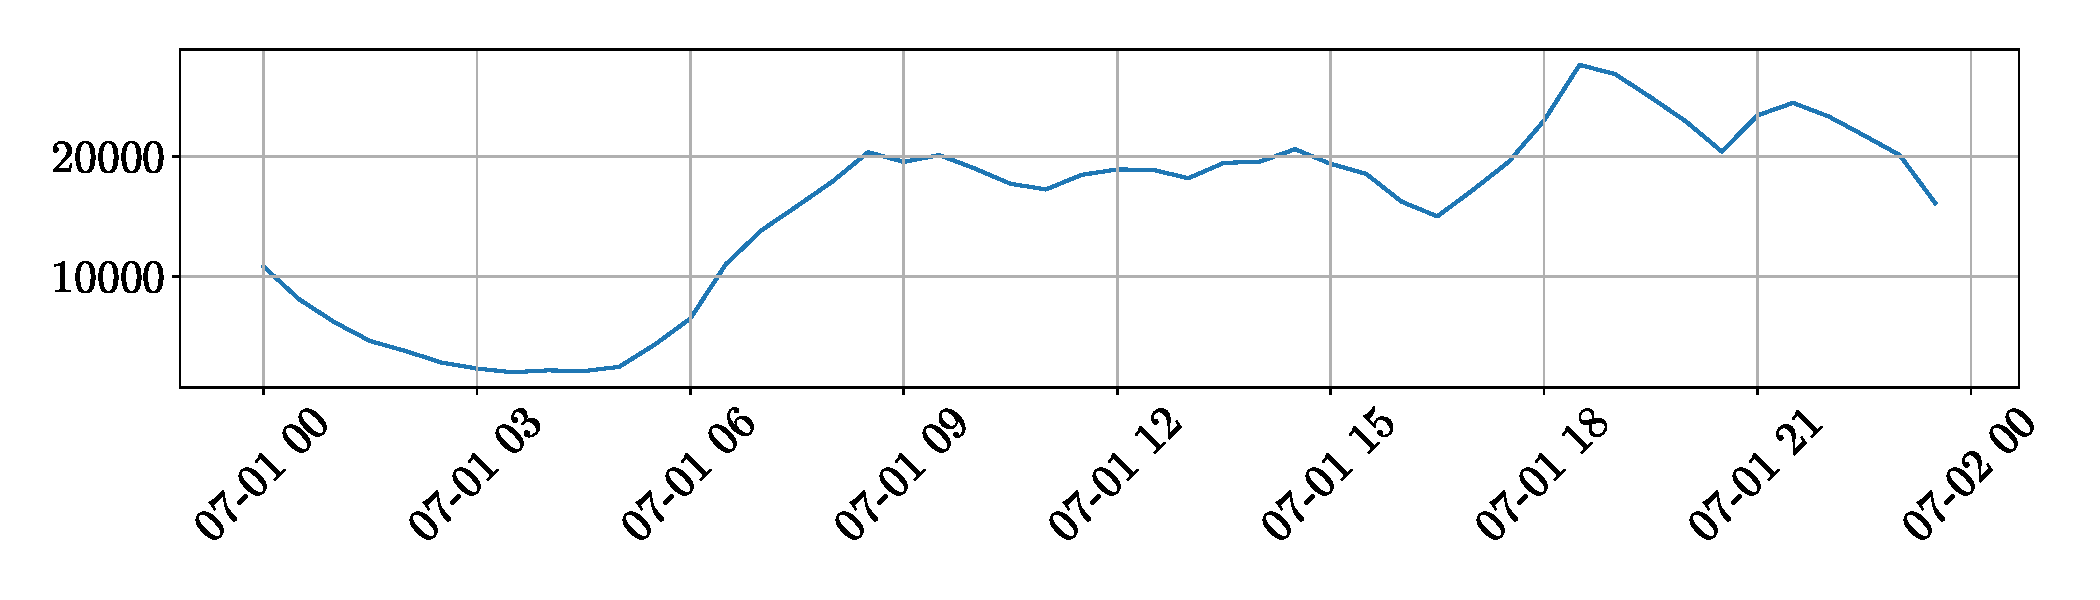
\includegraphics[width=0.7\linewidth]{./img/_ad_taxi_subset.pdf}
        \caption{Subset of the dataset}
    \end{figure}
\end{remark}

\begin{description}
    \item[Autocorrelation plot]
        Plot to visualize the correlation between nearby points of a series.
        Given the original series, it is duplicated, shifted by a lag $l$, and the Pearson correlation coefficient is then computed between the two series. This operation is repeated over different values of $l$.

        \begin{figure}[H]
            \centering
            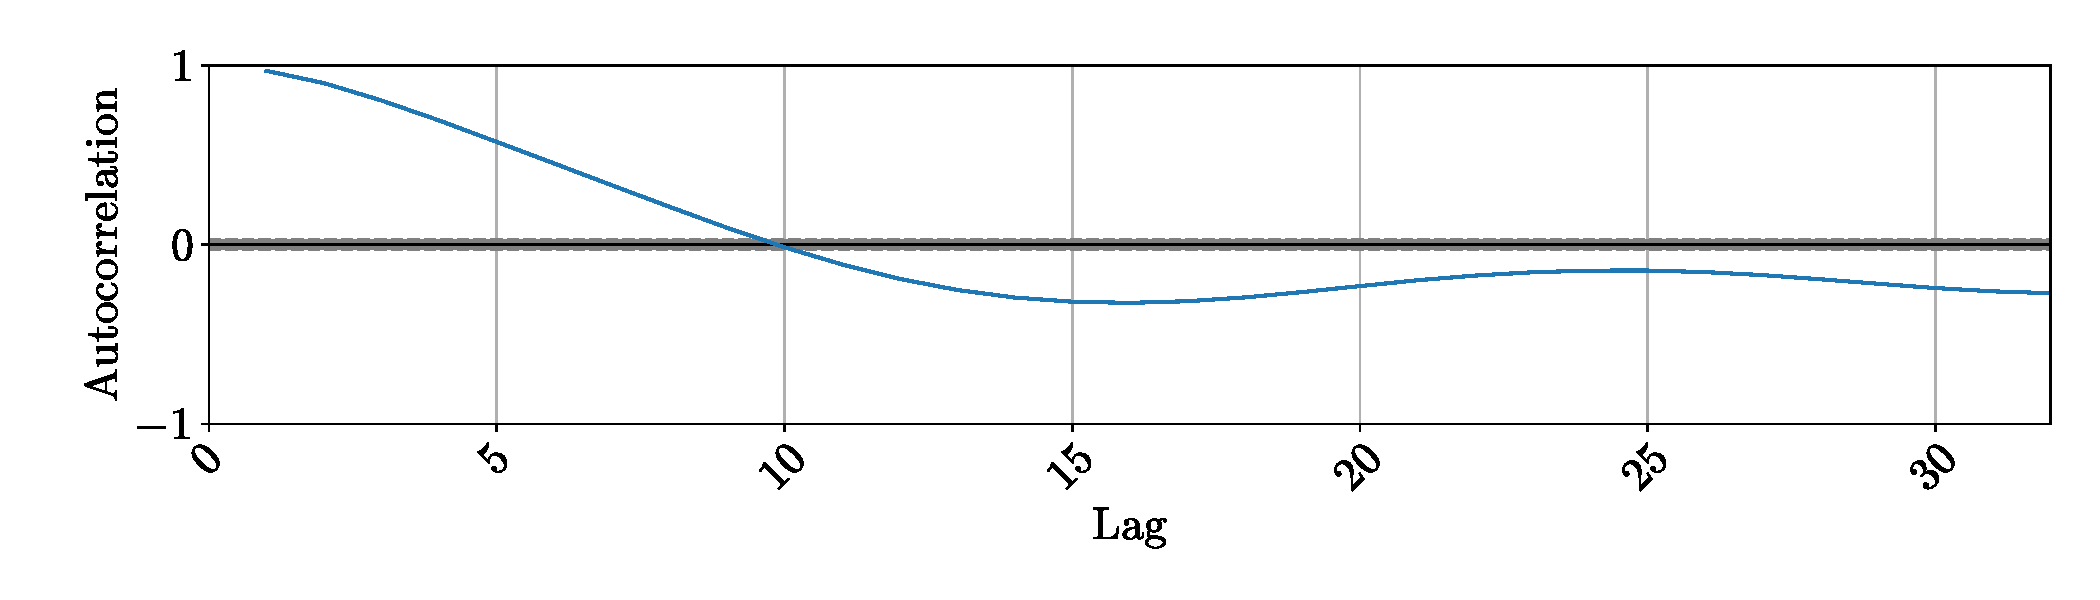
\includegraphics[width=0.7\linewidth]{./img/_ad_taxi_autocorrelation.pdf}
            \caption{
                \parbox[t]{0.6\linewidth}{
                    Autocorrelation plot of the subset of the dataset. There is strong correlation up to 4-5 lags.
                }
            }
        \end{figure}


    \item[Sliding window]
        Given a window size $w$ and a stride $s$, the dataset is split into sequences of $w$ continuous elements.

        \begin{remark}
            Incomplete sequences at the start and end of the dataset are ignored.
        \end{remark}

        \begin{remark}
            In \texttt{pandas}, the \texttt{rolling} method of \texttt{Dataframe} allows to create a slicing window iterator. This approach creates the windows row-wise and also considers incomplete windows.
            However, a usually more efficient approach is to construct the sequences column-wise by hand.
        \end{remark}

    \item[Multivariate KDE]
        Extension of KDE to vector variables.
\end{description}